\documentclass[border=2pt]{standalone}
\usepackage{tikz}
\begin{document}
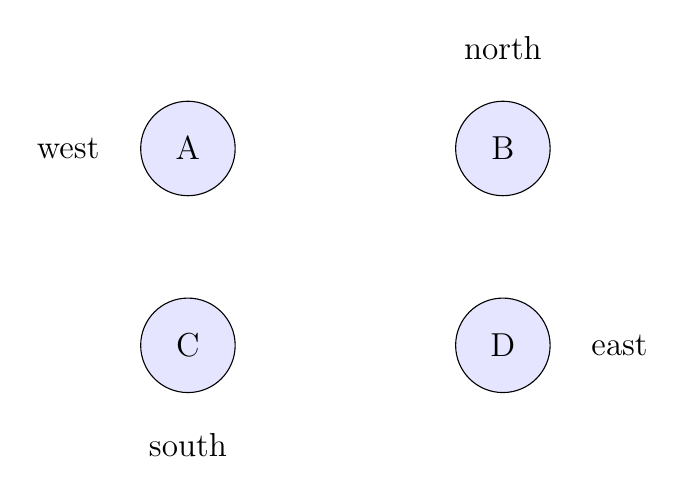
\begin{tikzpicture}[font=\large,state witness/.style={circle,draw,fill=blue!10,minimum size=12mm,outer sep=0pt}]
  \node[state witness] (A) at (0,0) {A};
  \node[state witness] (B) at (4,0) {B};
  \node[state witness] (C) at (0,-2.5) {C};
  \node[state witness] (D) at (4,-2.5) {D};
  \node[anchor=east] at (-1,0) {west};
  \node[anchor=south] at (4,1) {north};
  \node[anchor=north] at (0,-3.5) {south};
  \node[anchor=west] at (5,-2.5) {east};
\end{tikzpicture}
\end{document}
